\documentclass[a4paper]{article}

\usepackage{graphicx}          % For including graphics.
\usepackage{amsmath}           % Some mathematical symbols.

\addtolength{\topmargin}{-20mm}% Margin adjustments.
\addtolength{\textheight}{20mm}% Margin adjustments.

\begin{document}

\title{Image Enhancement Report\\
\large{EQ2330 Image and Video Processing, Project 1}}
\author{Harald Nordgren\\ haraldnordgren@gmail.com}
% \date{March 17, 2009} % Manual date

\maketitle

\section*{Summary}
\label{sec:summary}

I have investigated spatial and frequency domain image enhancement techniques in Matlab on the $512\times512$ demo image "Lena".

%Write a short summary of your report. Write approximately 150 words about the
%problem that you are considering, your solution, obtained results and the
%the conclusion. For example, this template provides instructions for writing the
%project reports for the EQ2330 Image Processing course. Read it thoroughly as it
%is expected that the instructions are followed.

\section{Introduction}
\label{sec:introduction}

This project was about restoring images the were degraded using three types of techniques.

The first sub-assigment deals with the dynamic range of greyscale images where intensity values are found in the range [0,255]. Looping over each pixel value and summing the pixel values into bins (one bin for all intensity values 0, one for 1, and so on) creates a histogram. A normal-looking image will have a histogram that uses the whole dynamic range and spreads somewhat evenly.

Using the function

\begin{equation}
	\label{dr}
	g(x, y) = min(max(\left\lfloor 0.2 \cdot  f (x, y) + 50 \right \rceil, 0), 255)
\end{equation}

the dynamic range can be lowered by squeezing the values together, resulting in a duller-looking image. Assuming an image that for some reason starts out with a small dynamic range, histogram equalization can stretch the dynamic range to the entire 8-bit spectrum, giving a more lively apperance. The cumulative sum of the normalized histogram for the low-contrast image can be calculated as follows

\begin{equation}
	s_k = 255 \sum_{j=0}^{k} p_r(r_j)
\end{equation}

where the dynamic range is stretched to [0,255] by multiplication with 255. p is the probability for each intensity value in the original image, and the sum for p over the entire numerical axis is 1 by definition. Mapping the intensity values of the low-contrast image to these summed values equalizes its histogram.

In the second sub-assignment, the \texttt{mynoisegen} function generates two types of noise that are applied to the original images, and I then attempt to recover that original. The Gaussian noise is additive, potentially giving values outside of [0,255], so the noised image is also requantized. The salt-and-pepper noise sets certain random pixels to 0 or 255, representing black and white, respectively, giving the impression that the image has been litteraly salted and peppered.

The attempts to recover the noised image realy on two very similar methods. The mean filter uses a kernel of a certain size (here a $3\times3$ matrix with every value equal to 1/9) which is convoluted with the noised image, effectively averaging each pixel value to that of its closest neighbors. The median filter replaces each pixel with the median of the neighboring pixels, meaning that these values have to be sorted first. Both methods remove high-frequency components from the images, meaning that noise is removed alongside some finer details of the original image.

In the final sub-assignment, the image is blurred by convoluting with a Gauss kernel generated by \texttt{myblurgen} and then quantized to give additive noise, modeled as

\begin{equation}
	f(x,y) = g(x,y) * h(x,y) + \eta(x,y)
\end{equation}

The task is then to deblur the image while only using the blurring function and the variance of the noise.

%Give an introduction to the problem considered. The introduction should be
%written such that it can be understood by an engineer whose area of expertise is
%not image processing. Motivate the problem by using references to work by other
%authors~\cite{coursebook}, as well as interesting applications.

%Define the mathematical notation used in the report and state the problem using
%this notation. Make sure that any assumptions you are using are explicit. It is
%often convenient to be able to refer to equations by numbers. An example
%equation is the additive noise degradation model for images

%\begin{equation}
%  \label{eqn:model}
%  g(x,y) = f(x,y) + \eta(x,y).
%\end{equation}

\section{System Description}
\label{sec:system}
In the first sub-assignment, I plotted the histogram for the three versions of the demo image, using \texttt{subplot}. To calculate histograms all matrices are first converted to an array vector with \texttt{(:)} and divided each value by the total sum before plotting as a bar graph.

To lower the contrast I iterated over each pixel and calculate \eqref{dr}, and to equalize the histogram I used \texttt{cumsum} and then mapped the low-contrast values to the summed function.

I used \texttt{mynoisegen} to add Gaussian and Salt-and-pepper noise to the original, and then tried removing it with mean and median filtering. The mean filter is quicker to calculate -- no sorting is needed -- but the median filter is likely to give slightly better results when dealing with outlier noise.

In the last task, I applied Gaussian blur by convolution the original images with a $8\times8$ kernel generated by \texttt{myblurgen}, and quantized the this image to 8-bit -- giving additive noise. Given the symmetry of the blur kernel (leading to a zero determinant) it is obvious that a simple inverse filter would not do. Using the variance of the quantization noise and the blurring function, I used \texttt{deconvwnr} to deblur the image.

To decrease ringings along the border of the image, I had to first run \texttt{edgetaper}. I then plotted the original, degenerated and deblurred images, along with their fourier spectra.

\section{Results}
\label{sec:results}

\begin{figure}[!ht]
  %\centering
  \centerline{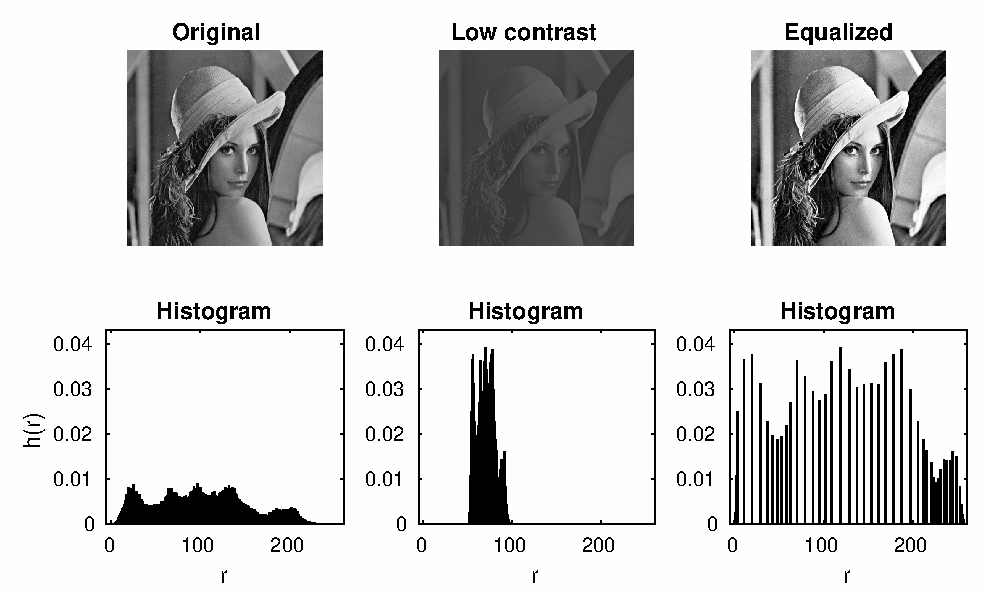
\includegraphics{images/2-1.eps}}
  \caption{Equalization}
  \label{fig:21}
\end{figure}
\begin{figure}[!ht]
  \centerline{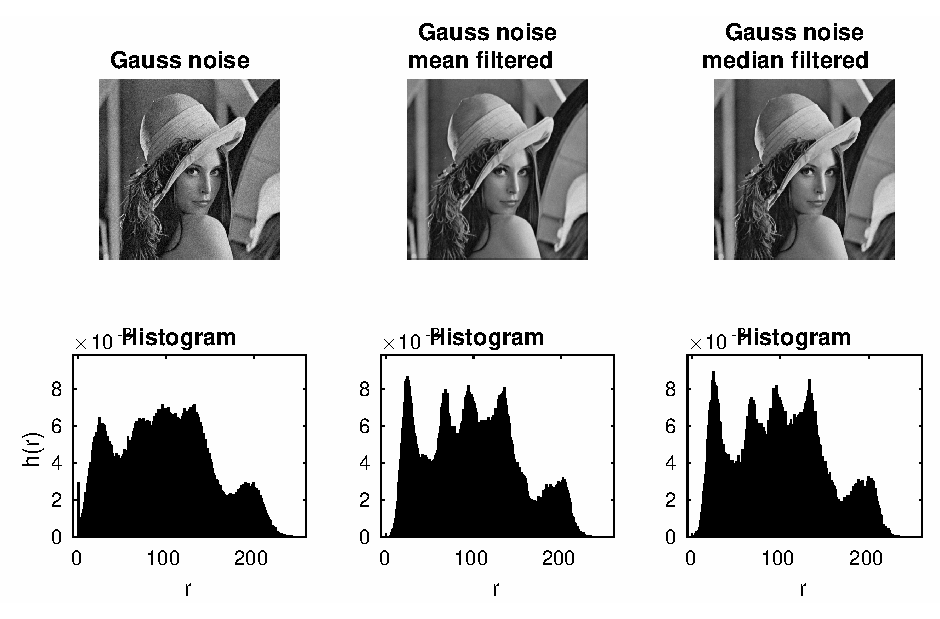
\includegraphics{images/2-2_gauss.eps}}
  \caption{Gauss noise}
  \label{fig:22g}
\end{figure}

The histogram for the low-contrast image (Figure~\ref{fig:21}) looks like what you would expect, squeezed togther, but still maintaining the overall shape. The low-contrast image looks almost like it is hidden behind a screen, and could be brought out by the correct means.

The equalized image looks great, maybe even better than the original, although the light areas are maybe  a bit too light, and edges, like the hat and its feather look overly sharp.

For a continuous probability density function we expect equalization to give a completely flat histogram, but for out quantized data it will show slight deviations from that but will be as close as possible.

The mean and median filters produced about the same result for the Gauss noise, which removes the noise while inducing some slight \textit{cel shading} or \textit{cartooninification} effect on the images.

\begin{figure}[!ht]
  %\centering
  \centerline{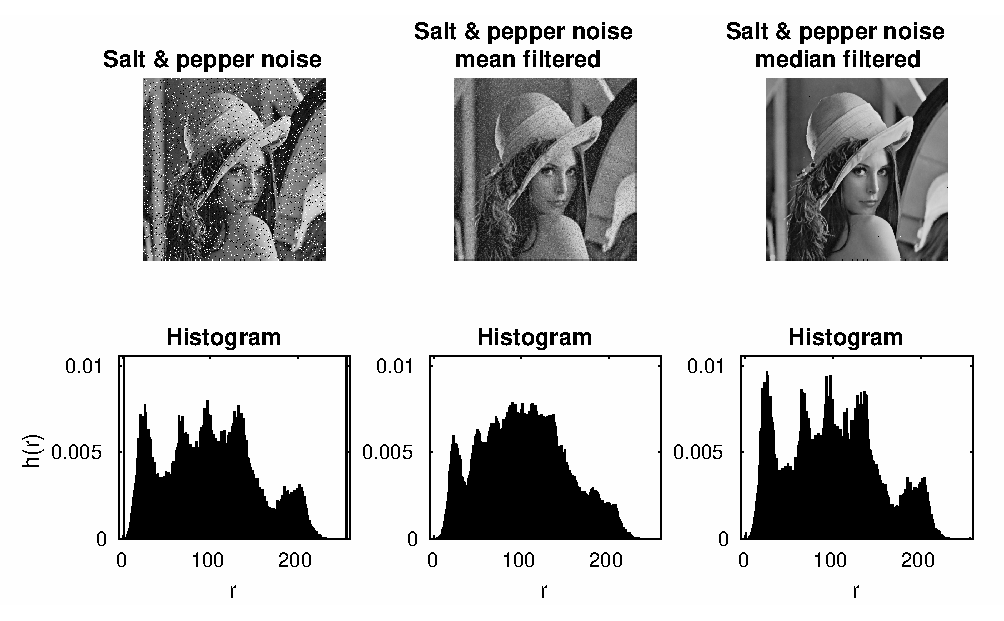
\includegraphics{images/2-2_saltp.eps}}
  \caption{Salt-and-pepper noise}
  \label{fig:22s}
\end{figure}
\begin{figure}[!ht]
  %\centering
  \centerline{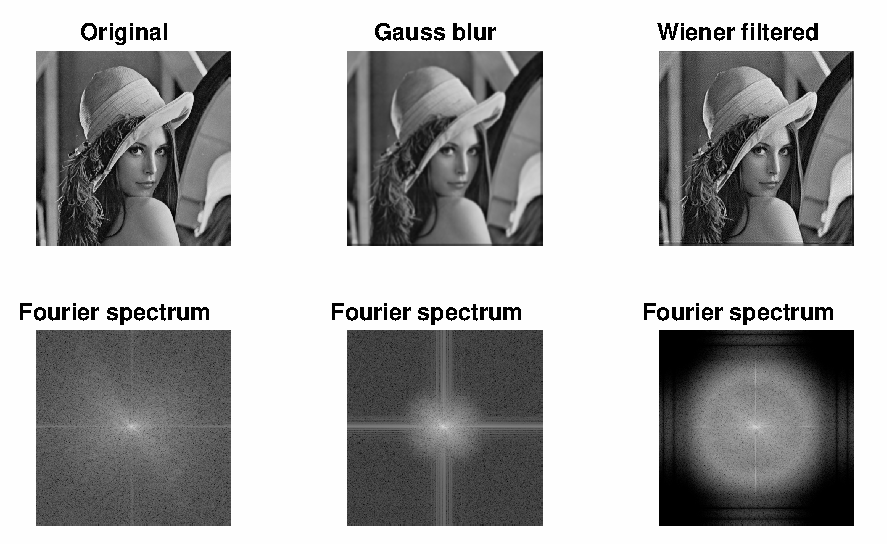
\includegraphics{images/3.eps}}
  \caption{Deblurring}
  \label{fig:3}
\end{figure}

Mean filtering does not produce a satisfying effect for the Salt-and-pepper noise. Although the image looks slighty better, it is heavily affected by the noise even after the filtering.

Surprisingly, the median filter produces almost perfect results for Salt-and-pepper noise, just missing a few spots, likely those where neighboring pixel were also noised, and on the borders where there are less non-affected pixels to pool information from.

The Wiener filter does an acceptable job on the blurred image (most likely the hardest one of the bunch), although there are circular artefact pattern all across the deblurred images, and straight lines along the edges. These lines were much worse without tapering, and perhaps could be entirely removed by a more precise algorithm.

\section*{Appendix}

\subsection*{MatLab code}
Here follows a condensed version of the Matlab code. I removed all \texttt{plotting}, \texttt{figures}, \texttt{subplots}, axis manipulation and \texttt{prints} for saving figures to file, but kept all the logic that enhances the images.
\begin{verbatim}
function assignment_2_1(image_path)

% ORIGINAL IMAGE

im = imread(image_path);
[rows, columns] = size(im);

im_hist = hist(im(:), 0:255);
normalized_im_hist = im_hist ./ sum(im_hist);

% LOW CONTRAST

a = 0.2;
b = 50;

im_lc = im;
for i = 1:rows
    for j = 1:columns
        im_lc(i,j) = min(max(round(a*im(i,j) + b), 0), 255);
    end
end

im_lc_hist = hist(im_lc(:), 0:255);
im_lc_hist_normalized = im_lc_hist ./ sum(im_lc_hist);


% HISTOGRAM EQUALIZATION

im_lc_hist_normalized_sum = 255 * cumsum(im_lc_hist_normalized);

im_lc_eq = im_lc;
for i = 1:rows
    for j = 1:columns
        im_lc_eq(i,j) = round(im_lc_hist_normalized_sum(im_lc(i,j)));
    end
end

im_lc_eq_hist = hist(im_lc_eq(:), 0:255);
im_lc_eq_hist_normalized = im_lc_eq_hist ./ sum(im_lc_eq_hist);

end



function assignment_2_2(image_path)

% ORIGINAL

im = imread(image_path);
[rows, columns] = size(im);


% GAUSS NOISE

gauss_noise = mynoisegen('gaussian', rows, columns, 0, 64);
im_gauss = uint8(min(max(round(double(im) + gauss_noise), 0), 255));


% GAUSS NOISE MEAN FILTERED

kernel = ones(3,3) / 9;
im_gauss_mean = uint8(round(conv2(double(im_gauss), kernel, 'same')));


% GAUSS NOISE MEDIAN FILTERED

im_gauss_median = medfilt2(im_gauss);


% SALT-N-PEPA

im_saltp = im;
n = mynoisegen('saltpepper', rows, columns, .05, .05);

im_saltp(n==0) = 0;
im_saltp(n==1) = 255;


% SALT & PEPPER NOISE MEAN FILTERED

im_saltp_mean = uint8(round(conv2(double(im_saltp), kernel, 'same')));


% SALT & PEPPER NOISE MEDIAN FILTERED

im_saltp_median = medfilt2(im_saltp);

end



function im_deblurred = deblur(im_blurry, h, noise_var)

im_blurry = double(im_blurry);
estimated_nsr = noise_var / var(im_blurry(:));

%Handles sharp edges
im_blurry_tapered = edgetaper(im_blurry, h);

im_deblurred = deconvwnr(im_blurry_tapered, h, estimated_nsr);

end



function assignment_3(image_path)


% ORIGINAL

im = double(imread(image_path));

im_fft = fft2(im);
im_fft_abs_log = log(abs(fftshift(im_fft)) + 1);
imshow(mat2gray(im_fft_abs_log));


% GAUSS BLURRED AND 8-BIT QUANTIZED

h = myblurgen('gaussian', 8);

im_conv = conv2(im, h, 'same');
im_conv_q = min(max(round(im_conv), 0), 255);

im_conv_q_fft = fft2(im_conv_q);
im_conv_q_fft_abs_log = log(abs(fftshift(im_conv_q_fft)) + 1);
imshow(mat2gray(im_conv_q_fft_abs_log));


% DEBLURRED IMAGE

diff_q = im_conv - im_conv_q;
var_q = var(diff_q(:));

im_deblurred = deblur(im_conv_q, h, var_q);

im_deblurred_fft = fft2(im_deblurred);
deblurred_fft_abs_log = log(abs(fftshift(im_deblurred_fft)) + 1);
imshow(mat2gray(deblurred_fft_abs_log));

end

\end{verbatim}

\end{document}
